\documentclass[11pt,a4paper]{article}

\usepackage[margin=1in]{geometry}
\usepackage{amsmath,amssymb}
\usepackage{booktabs}
\usepackage{longtable}
\usepackage{enumitem}
\usepackage{hyperref}
\usepackage{listings}
\usepackage{xcolor}
\usepackage{microtype}
\usepackage{tikz}
\usepackage{fancyvrb}
\usetikzlibrary{arrows.meta,positioning,shapes.geometric}

\hypersetup{
  colorlinks=true,
  linkcolor=blue!60!black,
  urlcolor=blue!60!black,
  pdftitle={Building Tiramisu From Scratch},
  pdfauthor={Tiramisu Project}
}

% Commit reference: short SHA + message
\newcommand{\commit}[2]{%
  \par\noindent\fbox{\parbox{\dimexpr\linewidth-2\fboxsep}{%
    \textbf{Git reference:} \texttt{#1} --- \emph{#2}}}%
  \par\smallskip
}

% After each code listing: what / design / why / math+perf (one paragraph)
\newcommand{\explain}{\par\smallskip\noindent}
\newcommand{\exhead}{\textbf{Reading this code.}\ }

\lstdefinestyle{cpp}{
  language=C++,
  basicstyle=\ttfamily\footnotesize,
  keywordstyle=\color{blue},
  commentstyle=\color{gray!70},
  stringstyle=\color{teal},
  showstringspaces=false,
  breaklines=true,
  frame=single,
  rulecolor=\color{black!20},
  backgroundcolor=\color{black!2},
  columns=fullflexible,
  keepspaces=true,
  tabsize=2,
  numbers=left,
  numberstyle=\tiny\color{gray},
  literate={->}{{$\rightarrow$}}1
}

\lstdefinestyle{cmake}{
  language=CMake,
  basicstyle=\ttfamily\footnotesize,
  breaklines=true,
  frame=single,
  rulecolor=\color{black!20},
  backgroundcolor=\color{black!2}
}

\lstdefinestyle{plain}{
  basicstyle=\ttfamily\footnotesize,
  breaklines=true,
  frame=single,
  rulecolor=\color{black!20},
  backgroundcolor=\color{black!2}
}

\title{\textbf{Building Tiramisu From Scratch}\\[0.4em]
\large A complete implementation guide for first-year CS students}
\author{}
\date{Repository HEAD: \texttt{cd6fabf} (\emph{batched matmul})}

\begin{document}
\maketitle

\begin{abstract}
\noindent
This document is a \textbf{standalone build guide}. A reader with C++20, linear algebra,
and basic calculus should be able to recreate the \textbf{tiramisu} machine learning
framework from an empty directory---without reading the source tree first.

\textbf{Prerequisites:} vectors, matrices, matrix multiply, partial derivatives, chain rule.
\textbf{Not required:} prior ML, PyTorch, or deep learning courses.

\textbf{Companion reference:} \texttt{docs/WIKI.md} (formulas, test map, known bugs).

\textbf{How to use this guide:} Build in the order of Sections~\ref{sec:timeline}--\ref{sec:gpt}
and Appendices~\ref{app:permute}--\ref{app:attention-shapes}. After each phase, write the
tests listed before moving on. Git commit SHAs mark when each capability landed in the real
repository (short hashes from \texttt{git log --oneline}).

\textbf{Reading convention:} Every code block is followed by a \textbf{Reading this code.}
paragraph covering what it does, design choices, why it is written that way, and the relevant
math or compiler/performance notes.

\textbf{Compile this document:}
\texttt{pdflatex BUILDING\_TIRAMISU.tex} (twice for TOC). Requires \texttt{listings},
\texttt{tikz}, \texttt{amsmath}.
\end{abstract}

\tableofcontents
\newpage

%==============================================================================
\section{Machine Learning in Plain Terms}
\label{sec:ml-intro}
%==============================================================================

\subsection{The Problem}

You have inputs $x$ (numbers) and want outputs $y$ (numbers). Example: $x$ is a
$28\times 28$ grayscale image (784 pixels), $y$ is the digit 0--9.

A hand-written program searches for pixel patterns. That fails on real-world data.

A \textbf{neural network} defines a \emph{family} of functions parameterized by millions
of adjustable numbers (\textbf{weights} / \textbf{parameters}). \textbf{Training} finds
parameter values that fit training examples.

\subsection{The Training Loop}

\begin{enumerate}[leftmargin=*]
  \item \textbf{Forward}: compute prediction $\hat{y} = f(x; \theta)$ with parameters $\theta$.
  \item \textbf{Loss}: scalar $L$ measuring error vs.\ true label $y$.
  \item \textbf{Backward}: compute $\partial L / \partial \theta_i$ for every parameter.
  \item \textbf{Update}: $\theta_i \leftarrow \theta_i - \eta \cdot \partial L / \partial \theta_i$
        (learning rate $\eta$).
\end{enumerate}

Repeat on many examples (an \textbf{epoch}) until $L$ stops decreasing.

\subsection{Gradients and the Chain Rule}

$\partial L / \partial w$ answers: if I nudge $w$ up slightly, does $L$ rise or fall?

For composed functions, the \textbf{chain rule} chains local derivatives:
\begin{equation}
  \frac{\partial L}{\partial w}
    = \frac{\partial L}{\partial z} \cdot \frac{\partial z}{\partial w}
\end{equation}
\textbf{Autograd} records the composition during forward and applies the chain rule
automatically in reverse.

\subsection{Tensors}

A \textbf{tensor} is a multi-dimensional array of numbers:

\begin{center}
\begin{tabular}{@{}clll@{}}
  \toprule
  Rank & Name & Shape example & Meaning \\
  \midrule
  0 & scalar & \texttt{\{1\}} & loss value \\
  1 & vector & \texttt{\{10\}} & class scores \\
  2 & matrix & \texttt{\{64, 784\}} & 64 images \\
  3 & 3-D & \texttt{\{32, 28, 784\}} & batch $\times$ seq $\times$ features \\
  \bottomrule
\end{tabular}
\end{center}

\textbf{Row-major (C) layout:} last index is fastest in memory. Shape \texttt{(2,3)} stores
\texttt{[a00,a01,a02,a10,a11,a12]} with strides \texttt{(3,1)}.

\subsection{What You Will Build}

Five static libraries, bottom to top:
\begin{lstlisting}[style=plain]
tiramisu_core     Storage, Tensor, dtype, device
tiramisu_ops      forward math (CPU, AVX2)
tiramisu_autograd differentiable wrappers + backward()
tiramisu_nn       Linear, Embedding, GPT, loss
tiramisu_optim    SGD, Adam
\end{lstlisting}
\explain\exhead This is the dependency stack you are implementing, not a single monolith.
\texttt{core} holds memory layout; \texttt{ops} performs numeric kernels with no knowledge of
training; \texttt{autograd} records how to differentiate those kernels; \texttt{nn} composes
them into layers; \texttt{optim} updates weights from \texttt{.grad()}. The design separates
\textbf{forward math} from \textbf{gradient bookkeeping} so you can test matmul correctness
before autograd exists, and test autograd on tiny graphs before building GPT. Dependencies flow
one way (upward only), which prevents circular includes and mirrors how PyTorch splits
\texttt{aten} (ops) from \texttt{autograd}. No compiler flags matter at this layer---it is
pure project structure.

End state: MNIST digit classifier + GPT-style transformer with working backward pass.

%==============================================================================
\section{Repository Evolution (Commit Timeline)}
\label{sec:timeline}
%==============================================================================

Build in this order. Commits are from the real \texttt{tiramisu} history:

\begin{center}
\small
\begin{longtable}{@{}clp{7.5cm}@{}}
  \toprule
  Order & SHA & Milestone \\
  \midrule
  \endhead
  1 & \texttt{36d5033} & Empty CMake project \\
  2 & \texttt{104ee1b} & \texttt{Storage} + aligned allocation + tests \\
  3 & \texttt{cbc4c3c} & \texttt{Tensor} views, strides, \texttt{permute} \\
  4 & \texttt{292d5aa} & Elementwise \texttt{ops} \\
  5 & \texttt{8619f91} & Library split: \texttt{core/}, \texttt{ops/} \\
  6 & \texttt{724a48a} & Autograd engine, \texttt{Node}, \texttt{backward()} \\
  7 & \texttt{d3ba005} & More autograd ops (\texttt{exp}, \texttt{relu}, \texttt{matmul}) \\
  8 & \texttt{8399e98} & \texttt{nn/} modules, \texttt{optim/}, \texttt{Linear} \\
  9 & \texttt{523814c} & MNIST example \\
  10 & \texttt{3cdc1e8} & \textbf{Bug fix:} \texttt{reduce\_grad\_to} for broadcast backward \\
  11 & \texttt{8423d3b} & Tiled SIMD matmul (AVX2) \\
  12 & \texttt{0a9d576} & \texttt{softmax}, \texttt{layernorm} \\
  13 & \texttt{cd6fabf} & Batched N-D matmul \\
  14 & (current tree) & Transformer stack: GELU, Embedding, MHA, GPT \\
  \bottomrule
\end{longtable}
\end{center}

%==============================================================================
\section{Project Scaffolding}
\label{sec:scaffold}
%==============================================================================

\commit{36d5033}{initial}

\subsection{Directory Layout}

Create this tree before writing logic:
\begin{lstlisting}[style=plain]
tiramisu/
  CMakeLists.txt
  core/
    CMakeLists.txt
    include/tiramisu/core/
    src/
  ops/
    CMakeLists.txt
    include/tiramisu/ops/
    cpu/
  autograd/
    CMakeLists.txt
    include/tiramisu/autograd/
    src/
  nn/
    CMakeLists.txt
    include/tiramisu/nn/
    src/
  optim/
    CMakeLists.txt
    include/tiramisu/optim/
    src/
  tests/
  examples/
\end{lstlisting}
\explain\exhead Each folder is one static library with a public \texttt{include/} and private
\texttt{src/}. Headers live under \texttt{include/tiramisu/<lib>/} so consumers write
\texttt{\#include "tiramisu/core/tensor.hpp"} without path collisions. \texttt{cpu/} under
\texttt{ops} leaves room for a future \texttt{cuda/} backend without touching autograd.
\texttt{tests/} and \texttt{examples/} are executables, not libraries---they link the stack
you build. This layout matches commit \texttt{8619f91} (\emph{architecture refactor}) when the
project split from a single folder into modules.

\subsection{Root \texttt{CMakeLists.txt}}

\begin{lstlisting}[style=cmake]
cmake_minimum_required(VERSION 3.20)
project(tiramisu LANGUAGES CXX)

set(CMAKE_CXX_STANDARD 20)
set(CMAKE_CXX_STANDARD_REQUIRED ON)
set(CMAKE_CXX_EXTENSIONS OFF)

option(TIRAMISU_BUILD_TESTS "Build unit tests" ON)
option(TIRAMISU_BUILD_EXAMPLES "Build examples" ON)

add_library(tiramisu_warnings INTERFACE)
target_compile_options(tiramisu_warnings INTERFACE
  -Wall -Wextra -Wpedantic -Wshadow)

add_subdirectory(core)
add_subdirectory(ops)
add_subdirectory(autograd)
add_subdirectory(nn)
add_subdirectory(optim)

if(TIRAMISU_BUILD_TESTS)
  enable_testing()
  include(FetchContent)
  FetchContent_Declare(googletest
    GIT_REPOSITORY https://github.com/google/googletest.git
    GIT_TAG v1.15.2)
  FetchContent_MakeAvailable(googletest)
  add_subdirectory(tests)
endif()
\end{lstlisting}
\explain\exhead CMake declares C++20, wires five \texttt{add\_subdirectory} calls in
\textbf{dependency order} (\texttt{core} first), and fetches GoogleTest only when tests are on.
\texttt{tiramisu\_warnings} is an INTERFACE library so every target gets \texttt{-Wall -Wextra}
without copy-pasting flags---a common CMake pattern for consistent diagnostics. Sanitizers
(not shown here; see root \texttt{CMakeLists.txt} in the repo) attach only in Debug because
ASan slows training loops. \texttt{FetchContent} for GTest avoids requiring system packages on
lab machines. Compiler optimization (\texttt{-O3 -mavx2}) is applied \emph{per library} in
\texttt{ops/CMakeLists.txt}, not globally, so Debug builds stay fast to compile while matmul
still runs fast in Release.

\subsection{Dependency Graph}

\begin{center}
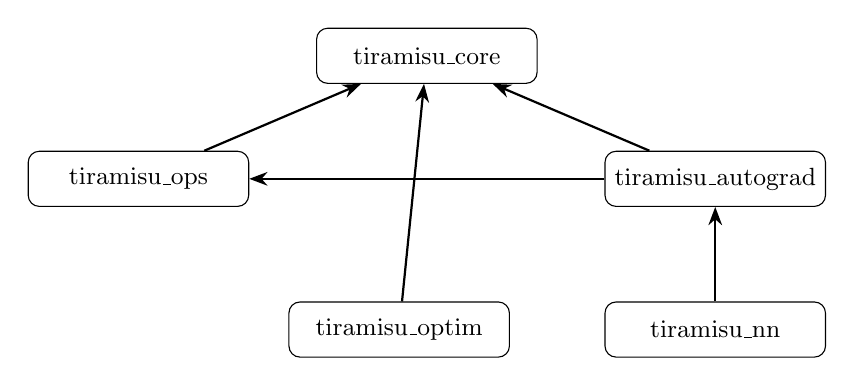
\begin{tikzpicture}[
  node distance=1.2cm,
  lib/.style={rectangle, draw, rounded corners, minimum width=2.8cm,
              minimum height=0.7cm, font=\small},
  arr/.style={-{Stealth}, thick}
]
  \node[lib] (core) {tiramisu\_core};
  \node[lib, below left=of core] (ops) {tiramisu\_ops};
  \node[lib, below right=of core] (autograd) {tiramisu\_autograd};
  \node[lib, below=of autograd] (nn) {tiramisu\_nn};
  \node[lib, left=of nn] (optim) {tiramisu\_optim};
  \draw[arr] (ops) -- (core);
  \draw[arr] (autograd) -- (core);
  \draw[arr] (autograd) -- (ops);
  \draw[arr] (nn) -- (autograd);
  \draw[arr] (optim) -- (core);
\end{tikzpicture}
\end{center}

\explain\exhead Arrows point from dependent to dependency: \texttt{nn} needs autograd, autograd
needs ops and core, optim only needs core (reads raw tensor data). This DAG prevents circular
includes---if \texttt{ops} imported autograd, matmul would depend on graph code and you could not
unit-test forward kernels in isolation. \texttt{optim} deliberately does not link autograd: it
only mutates \texttt{.data()} after gradients are already computed.

\textbf{Rule:} \texttt{ops} never includes autograd. \texttt{nn} never calls \texttt{ops::}
directly---only \texttt{autograd::}.

%==============================================================================
\section{Phase 1: Core --- Storage and Tensor}
\label{sec:core}
%==============================================================================

\commit{104ee1b}{storage implementation \& tests}
\commit{cbc4c3c}{tensor stuff}

\subsection{Step 1.1: \texttt{DType} and \texttt{Device}}

File \texttt{core/include/tiramisu/core/dtype.hpp}:
\begin{lstlisting}[style=cpp]
enum class DType { Float32, Int32 };

template<typename T> DType dtype_of();
template<> inline DType dtype_of<float>() { return DType::Float32; }

inline std::size_t dtype_size(DType dt) {
  switch (dt) {
    case DType::Float32: return 4;
    case DType::Int32:   return 4;
  }
  throw std::runtime_error("unknown dtype");
}
\end{lstlisting}
\explain\exhead \texttt{DType} tags every buffer so \texttt{Storage} knows element size and
\texttt{Tensor::data<float>()} can reject wrong template instantiations at runtime. The
\texttt{dtype\_of<T>()} trait maps C++ types to enums at compile time---no virtual dispatch.
We only implement \texttt{Float32} in hot paths today; \texttt{Int32} exists for future index
tensors. Design choice: keep dtypes minimal rather than supporting every NumPy dtype on day
one. Math: allocation size is $\text{numel} \times \texttt{dtype\_size}(dt)$ bytes; for
\texttt{Float32} that is $4n$.

\texttt{Device} is an enum with \texttt{CPU} only for now.

\subsection{Step 1.2: \texttt{Storage}}

Owns bytes. \textbf{Non-copyable}---ownership via \texttt{shared\_ptr} on tensors.

\begin{lstlisting}[style=cpp]
// core/include/tiramisu/core/storage.hpp
class Storage {
 public:
  Storage(std::size_t count, DType dtype, Device device,
          std::size_t alignment = 64);
  ~Storage();
  Storage(const Storage&) = delete;
  Storage& operator=(const Storage&) = delete;

  std::byte* data();
  const std::byte* data() const;
  std::size_t numel() const;
  std::size_t nbytes() const;
  DType dtype() const;
  Device device() const;
 private:
  std::byte* data_ = nullptr;
  std::size_t count_ = 0;
  DType dtype_;
  Device device_;
  std::size_t alignment_;
};
\end{lstlisting}
\explain\exhead \texttt{Storage} is the \textbf{sole owner} of heap bytes. Tensors only borrow
via \texttt{shared\_ptr}. Copy is deleted so you cannot accidentally double-free or have two
owners with divergent lifetimes. \texttt{numel()} counts elements; \texttt{nbytes()} is
$\text{numel} \times \texttt{dtype\_size}$. The default 64-byte alignment matches AVX-512 cache
line conventions and satisfies \texttt{aligned\_alloc} requirements (size must be a multiple
of alignment). This type knows nothing about shape---shape is entirely a \texttt{Tensor} concern,
which keeps storage reusable for raw buffers.

Allocation (\texttt{core/src/storage.cpp})---use \texttt{aligned\_alloc} for SIMD:
\begin{lstlisting}[style=cpp]
Storage::Storage(std::size_t count, DType dtype, Device device,
                 std::size_t alignment)
    : count_(count), dtype_(dtype), device_(device), alignment_(alignment) {
  assert((alignment & (alignment - 1)) == 0);  // power of 2
  if (count == 0) { data_ = nullptr; return; }
  std::size_t bytes = count * dtype_size(dtype);
  std::size_t alloc_size = (bytes + alignment - 1) & ~(alignment - 1);
  data_ = static_cast<std::byte*>(std::aligned_alloc(alignment, alloc_size));
  if (!data_) throw std::bad_alloc();
}
\end{lstlisting}
\explain\exhead The constructor allocates $\lceil \text{bytes} / \text{align} \rceil \times
\text{align}$ bytes using bit-masking (\texttt{\& \textasciitilde(alignment-1)}), which is the
standard round-up for power-of-two alignments. The assert enforces power-of-two alignment as
required by POSIX \texttt{aligned\_alloc}. Empty tensors (\texttt{count == 0}) get
\texttt{nullptr}---valid for scalar edge cases. \textbf{Why aligned?} Later, \texttt{ops} uses
AVX2 \texttt{\_mm256\_loadu\_ps}; aligned allocation helps when you switch to aligned loads
for marginal gains. \texttt{-O3} on \texttt{ops} will vectorize elementwise loops over
contiguous buffers; aligned base pointers improve store merging. No math beyond byte counting
here.

\subsection{Step 1.3: \texttt{Tensor} as a View}

\textbf{Critical design:} \texttt{Tensor} does \textbf{not} own memory.

\begin{lstlisting}[style=cpp]
// core/include/tiramisu/core/tensor.hpp (essential API)
class Tensor {
 public:
  Tensor(std::vector<int64_t> shape, DType dtype = DType::Float32,
         Device device = Device::CPU);
  Tensor(std::shared_ptr<Storage> storage, std::vector<int64_t> shape,
         std::vector<int64_t> strides, std::size_t offset);

  const std::vector<int64_t>& shape() const;
  const std::vector<int64_t>& strides() const;
  int64_t numel() const;
  bool is_contiguous() const;

  template<typename T> T* data();
  template<typename T> T& at(std::initializer_list<int64_t> indices);

  Tensor view(std::vector<int64_t> new_shape) const;
  Tensor reshape(std::vector<int64_t> new_shape) const;
  Tensor permute(std::vector<int64_t> dims) const;
  Tensor transpose(int64_t dim0, int64_t dim1) const;
  Tensor contiguous() const;
  Tensor slice(int64_t dim, int64_t start, int64_t end) const;

  bool requires_grad() const;
  void set_requires_grad(bool r);
  const std::shared_ptr<Tensor>& grad() const;
  const std::shared_ptr<Node>& grad_fn() const;
  void set_grad_fn(std::shared_ptr<Node> fn);
  void accumulate_grad(const Tensor& g);

 private:
  std::shared_ptr<Storage> storage_;
  std::vector<int64_t> shape_, strides_;
  std::size_t offset_ = 0;
  struct AutogradState {
    bool requires_grad = false;
    std::shared_ptr<Tensor> grad;
    std::shared_ptr<Node> grad_fn;
  };
  std::shared_ptr<AutogradState> autograd_state_;
};
\end{lstlisting}
\explain\exhead A \texttt{Tensor} is a \textbf{view}: \texttt{(storage, shape, strides, offset)}
interprets the same bytes under different shapes. Two constructors exist---allocate fresh
(\texttt{shape} only) or alias existing storage (internal views). \texttt{AutogradState} is
behind a \texttt{shared\_ptr} so copying a \texttt{Tensor} handle shares \texttt{grad} and
\texttt{grad\_fn}; this is how residual connections accumulate gradients into the same buffer.
Design tradeoff: autograd metadata lives on the tensor, not a separate tape object, keeping
the implementation small. Index math:
$\text{idx} = \text{offset} + \sum_i c_i \cdot \text{stride}_i$.

\subsubsection{Contiguous Strides}

\begin{lstlisting}[style=cpp]
std::vector<int64_t> contiguous_strides(const std::vector<int64_t>& shape) {
  std::vector<int64_t> strides(shape.size());
  int64_t s = 1;
  for (int i = (int)shape.size() - 1; i >= 0; --i) {
    strides[i] = s;
    s *= shape[i];
  }
  return strides;
}
\end{lstlisting}
\explain\exhead For row-major (C) layout, the last dimension has stride 1 and each earlier stride
is the product of later shapes: $\sigma_i = \prod_{j>i} s_j$. Example: shape \texttt{(2,3)}
$\Rightarrow$ strides \texttt{(3,1)}. This makes flat index $i = c_0 \cdot 3 + c_1$.
\texttt{is\_contiguous()} compares live strides to this formula---if they match, SIMD kernels
can walk memory sequentially. Non-contiguous tensors (after \texttt{permute}) need gather loops
or a \texttt{contiguous()} copy before AVX2 matmul.

For shape \texttt{(2,3)}: strides \texttt{(3,1)}. Flat index:
$\mathrm{idx} = \mathrm{offset} + \sum_i c_i \cdot \mathrm{stride}_i$.

\subsubsection{Fresh Tensor Constructor}

\begin{lstlisting}[style=cpp]
Tensor::Tensor(std::vector<int64_t> shape, DType dtype, Device device)
    : shape_(std::move(shape)), offset_(0) {
  strides_ = contiguous_strides(shape_);
  storage_ = std::make_shared<Storage>(numel(), dtype, device);
}
\end{lstlisting}
\explain\exhead This is the user-facing constructor: supply a shape, get a dense zero-initialized
buffer (you may add explicit zero-fill; uninitialized memory is a common student bug). It
computes $\text{numel} = \prod_i s_i$, allocates one \texttt{Storage} of that many elements,
and sets row-major strides. One allocation per new tensor---views created later add zero
allocations. Compiler: \texttt{numel()} is inlineable; no optimization yet beyond what
\texttt{-O2} gives the constructor itself.

\subsubsection{Negative Dimension Indexing}

\texttt{permute} and \texttt{transpose} accept negative dims: \texttt{dim=-1} means last
axis. Normalize with \texttt{dim += rank} before bounds checks. This matches NumPy/PyTorch
ergonomics so \texttt{transpose(k, -1)} in attention does not need manual rank arithmetic.

\subsubsection{\texttt{permute} --- No Copy}

Only permutes \texttt{shape\_} and \texttt{strides\_}. Example: \texttt{(2,3,4)} with
strides \texttt{(12,4,1)}, \texttt{transpose(0,1)} $\rightarrow$ shape \texttt{(3,2,4)},
strides \texttt{(4,12,1)}. Memory cost is zero; you are editing metadata on the stack. Kernels
that assume contiguous layout must not call \texttt{data()} blindly after permute---call
\texttt{contiguous()} first or use stride-aware indexing like \texttt{apply\_binary\_op}.

\subsubsection{\texttt{reshape} = \texttt{contiguous().view()}}

May allocate if input is non-contiguous because \texttt{view} requires dense row-major layout
with $\text{numel}(\text{new\_shape}) = \text{numel}(\text{old})$. Design: reshape is ``make
contiguous if needed, then reinterpret bytes''---not a free view on transposed tensors.

\subsubsection{\texttt{accumulate\_grad}}

Gradients \textbf{add} when a tensor is used twice (residual connections):
\begin{lstlisting}[style=cpp]
void Tensor::accumulate_grad(const Tensor& g) {
  Tensor c_g = g.contiguous();
  if (!autograd_state_->grad) {
    Tensor new_grad(c_g.shape(), c_g.dtype(), c_g.device());
    std::copy(c_g.data<float>(), c_g.data<float>() + c_g.numel(),
              new_grad.data<float>());
    autograd_state_->grad = std::make_shared<Tensor>(new_grad);
  } else {
    float* cur = autograd_state_->grad->data<float>();
    const float* inc = c_g.data<float>();
    for (int64_t i = 0; i < autograd_state_->grad->numel(); ++i)
      cur[i] += inc[i];
  }
}
\end{lstlisting}
\explain\exhead During backward, a tensor may receive gradients from \textbf{multiple children}
(e.g.\ $x$ in $x + f(x)$). \texttt{accumulate\_grad} adds incoming grads elementwise:
$\text{grad} \leftarrow \text{grad} + g$. First call allocates \texttt{grad}; later calls
add in place. We \texttt{contiguous()} the incoming grad because upstream ops may return
strided views. Without accumulation, the second path's gradient would overwrite the first---residual
networks would train incorrectly. Math is vector addition over $\mathbb{R}^n$; a smart compiler
could auto-vectorize the loop with \texttt{-O3 -ffast-math}, but we keep it explicit for clarity.

\subsection{Step 1.4: Tests to Write First}

From \texttt{tests/core/tensor\_test.cpp}:
\begin{lstlisting}[style=cpp]
TEST(TensorUtils, ContiguousStrides) {
  EXPECT_EQ(tiramisu::contiguous_strides({3, 4}),
            std::vector<int64_t>({4, 1}));
}

TEST(TensorTest, TransposeAndPermute) {
  tiramisu::Tensor t({2, 3, 4});
  auto trans = t.transpose(0, 1);
  EXPECT_EQ(trans.shape(), std::vector<int64_t>({3, 2, 4}));
  EXPECT_EQ(trans.strides(), std::vector<int64_t>({4, 12, 1}));
}
\end{lstlisting}
\explain\exhead Tests pin down \textbf{metadata invariants}, not just values. After
\texttt{transpose(0,1)} on shape \texttt{(2,3,4)}, strides must become \texttt{(4,12,1)}---if
you accidentally recomputed contiguous strides from the new shape, transposes would silently
copy or corrupt indexing. These tests cost milliseconds and prevent week-long autograd bugs.
No performance angle: tests run in Debug without AVX flags.

Run: \texttt{cmake -S . -B build \&\& cmake --build build \&\& ctest --test-dir build}

%==============================================================================
\section{Phase 2: Forward Ops}
\label{sec:ops}
%==============================================================================

\commit{292d5aa}{basic ops}
\commit{8619f91}{architecture refactor}

\subsection{Step 2.1: \texttt{broadcast\_shapes}}

File \texttt{ops/cpu/broadcast.cpp}:
\begin{lstlisting}[style=cpp]
std::vector<int64_t> broadcast_shapes(const std::vector<int64_t>& a,
                                      const std::vector<int64_t>& b) {
  int64_t rank_a = a.size(), rank_b = b.size();
  int64_t out_rank = std::max(rank_a, rank_b);
  std::vector<int64_t> out(out_rank);
  for (int64_t i = 0; i < out_rank; ++i) {
    int64_t da = (i < out_rank - rank_a) ? 1 : a[i - (out_rank - rank_a)];
    int64_t db = (i < out_rank - rank_b) ? 1 : b[i - (out_rank - rank_b)];
    if (da != db && da != 1 && db != 1)
      throw std::invalid_argument("not broadcastable");
    out[i] = std::max(da, db);
  }
  return out;
}
\end{lstlisting}
\explain\exhead Implements NumPy broadcasting \textbf{shape rules only}---no data movement.
Left-padding with implicit 1s is done by indexing operands from the right inside the loop.
Output dim is $\max(a_i,b_i)$; incompatible if $a_i \neq b_i$ and neither is 1. Centralizing
this function (commit \texttt{292d5aa}) means elementwise ops and batched matmul share identical
semantics. Called once per op, not per element---negligible vs.\ the compute loop.

\subsection{Step 2.2: Elementwise Engine with Stride-0 Broadcast}

\textbf{Key trick:} dimension of size 1 gets stride 0.

\begin{lstlisting}[style=cpp]
void pad_to_rank(const std::vector<int64_t>& shape,
                 const std::vector<int64_t>& strides, int64_t target_rank,
                 std::vector<int64_t>& out_shape,
                 std::vector<int64_t>& out_strides) {
  out_shape.resize(target_rank, 1);
  out_strides.resize(target_rank, 0);
  int64_t diff = target_rank - (int64_t)shape.size();
  for (size_t i = 0; i < shape.size(); ++i) {
    out_shape[diff + i] = shape[i];
    out_strides[diff + i] = (shape[i] == 1) ? 0 : strides[i];
  }
}
\end{lstlisting}
\explain\exhead Before the main loop, both operands are \textbf{virtually padded} to the output
rank. Crucially, any dimension of size 1 gets \textbf{stride 0}: advancing along that axis
does not move the pointer, so one bias element is reused for all batch rows without allocating
a \texttt{(64,10)} expanded copy. Design: one generic \texttt{apply\_binary\_op} template
avoids duplicating add/mul/div loops. Math: $y_i = op(a_i, b_i)$ with $a_i,b_i$ fetched via
strided indexing. The hot loop is branch-light; with \texttt{-O3 -mavx2} on \texttt{ops},
\texttt{apply\_unary\_op} over contiguous data auto-vectorizes to 8-wide SIMD; binary broadcast
loops are harder to vectorize due to irregular strides.

Loop over output flat index $i$, decode coordinates, index into $a$ and $b$:
\begin{lstlisting}[style=cpp]
Tensor add(const Tensor& a, const Tensor& b) {
  return apply_binary_op(a, b, [](float x, float y) { return x + y; });
}
Tensor relu(const Tensor& t) {
  return apply_unary_op(t, [](float x) { return std::max(0.f, x); });
}
\end{lstlisting}
\explain\exhead \texttt{add}/\texttt{relu} are thin wrappers---the engine does the work.
\texttt{add}: $y_i = a_i + b_i$. \texttt{relu}: $y_i = \max(0, x_i)$, a piecewise linear
activation that zeroes negative inputs (kills gradient there in backward). Unary ops call
\texttt{contiguous()} first because the simple loop assumes stride-1 layout. Design: lambdas
keep one loop implementation; compiler inlines them at \texttt{-O3}.

\textbf{GELU} (needed later for GPT-2-style FFN):
\begin{equation}
  \mathrm{GELU}(x) = \frac{x}{2}\left(1 + \tanh\left(\sqrt{\tfrac{2}{\pi}}(x + 0.044715\,x^3)\right)\right)
\end{equation}
\begin{lstlisting}[style=cpp]
Tensor gelu(const Tensor& t) {
  return apply_unary_op(t, [](float x) {
    constexpr float k = 0.7978845608f;  // sqrt(2/pi)
    float x3 = x * x * x;
    return 0.5f * x * (1.0f + std::tanh(k * (x + 0.044715f * x3)));
  });
}
\end{lstlisting}
\explain\exhead GELU is a smooth alternative to ReLU used in GPT-2 FFN layers. The tanh
approximation avoids the error function $\mathrm{erf}$ and is standard in production transformers.
Constants: $k = \sqrt{2/\pi} \approx 0.7979$. Backward (later in autograd) must snapshot
input $x$ because the derivative involves $\tanh$ and $x^2$ terms. Forward is elementwise;
\texttt{std::tanh} may not vectorize as cleanly as \texttt{exp}, but FFN is a smaller fraction
of attention cost.

\subsection{Step 2.3: Reduce Ops}

\begin{lstlisting}[style=cpp]
Tensor sum(const Tensor& t) {
  Tensor out({1});
  float s = 0.f;
  Tensor c = t.contiguous();
  for (int64_t i = 0; i < c.numel(); ++i) s += c.data<float>()[i];
  out.data<float>()[0] = s;
  return out;
}
\end{lstlisting}
\explain\exhead \texttt{sum} collapses all elements to one scalar: $S = \sum_i x_i$. Output shape
\texttt{\{1\}} matches loss tensors used in \texttt{backward(loss)}. We contiguous-copy first so
the reduction loop is a single stride-1 pass---amenable to SIMD horizontal add if you optimize
later. \texttt{mean} divides by $N$; cross-entropy and loss averaging use this. Reduction is
$O(n)$; memory $O(1)$ output.

\subsection{Step 2.4: Ops CMake}

\begin{lstlisting}[style=cmake]
add_library(tiramisu_ops cpu/elementwise.cpp cpu/reduce.cpp
                        cpu/broadcast.cpp cpu/matmul.cpp
                        cpu/normalization.cpp)
target_compile_options(tiramisu_ops PRIVATE -O3 -mavx2 -mfma)
target_link_libraries(tiramisu_ops PUBLIC tiramisu_core)
\end{lstlisting}
\explain\exhead \texttt{-O3} enables aggressive inlining and loop vectorization on kernels.
\texttt{-mavx2 -mfma} unlocks 256-bit SIMD and fused multiply-add for matmul tiles (commit
\texttt{8423d3b}). Applied \textbf{only} to \texttt{tiramisu\_ops} so Debug builds of tests stay
quick while Release matmul is fast. \texttt{-mfma} maps $c \leftarrow c + a \times b$ to one
instruction---critical in the inner GEMM tile. OpenMP (optional in repo) can parallelize batch
slices across cores.

%==============================================================================
\section{Phase 3: Autograd Engine}
\label{sec:autograd}
%==============================================================================

\commit{724a48a}{autograd}
\commit{d3ba005}{expanding autograd}
\commit{3cdc1e8}{broadcast reduction bug fixed}

\subsection{Step 3.1: \texttt{Node}}

\begin{lstlisting}[style=cpp]
// core/include/tiramisu/core/node.hpp
struct Node {
  std::vector<Tensor> inputs;
  std::function<std::vector<Tensor>(const Tensor& grad_output)> backward_fn;
};
\end{lstlisting}
\explain\exhead A \texttt{Node} is one edge in the computation graph: it remembers parent
\texttt{inputs} and a \texttt{backward\_fn} that maps upstream gradient $\partial L/\partial y$
to gradients w.r.t.\ each input. Using \texttt{std::function} trades a small virtual-call overhead
for simplicity---no \texttt{Function} subclass hierarchy. Design: graph is implicit in tensors
(\texttt{grad\_fn} pointers), not a separate tape object. Memory: lambdas may capture tensors
by value (copy handles sharing storage), which keeps backward closures alive after forward
returns.

\subsection{Step 3.2: Wrapper Pattern (Every Differentiable Op)}

\begin{lstlisting}[style=cpp]
Tensor add(const Tensor& a, const Tensor& b) {
  Tensor out = tiramisu::ops::add(a, b);
  if (grad_enabled() && (a.requires_grad() || b.requires_grad())) {
    auto node = std::make_shared<Node>();
    node->inputs = {a, b};
    node->backward_fn = [a, b](const Tensor& grad_out) {
      return std::vector<Tensor>{
        reduce_grad_to(grad_out, a.shape()),
        reduce_grad_to(grad_out, b.shape())};
    };
    out.set_requires_grad(true);
    out.set_grad_fn(node);
  }
  return out;
}
\end{lstlisting}
\explain\exhead Pattern for \textbf{every} differentiable op: (1) call \texttt{ops::} for forward,
(2) if grad mode on and any input tracks grad, attach a \texttt{Node}. For \texttt{add},
$\partial L/\partial a = \partial L/\partial c$ and same for $b$---but only after
\texttt{reduce\_grad\_to} if shapes were broadcast. We gate on \texttt{grad\_enabled()} so
inference and \texttt{gradcheck} finite-difference passes do not build graphs. Why separate
\texttt{ops} and \texttt{autograd}? Forward kernels stay testable without autograd; autograd
never reimplements matmul, only its backward rule.

\subsection{Step 3.3: \texttt{reduce\_grad\_to} --- Do Not Skip}

\commit{3cdc1e8}{broadcast reduction bug fixed}

When forward broadcasts \texttt{(64,10) + (10,)}, backward gets grad \texttt{(64,10)} but
bias needs \texttt{(10,)}:
\begin{equation}
  \frac{\partial L}{\partial b_j} = \sum_{i=0}^{63} \frac{\partial L}{\partial y_{i,j}}
\end{equation}

\begin{lstlisting}[style=cpp]
static Tensor reduce_grad_to(const Tensor& grad,
                             const std::vector<int64_t>& target_shape) {
  if (grad.shape() == target_shape) return grad;
  Tensor result = grad.contiguous();
  while (result.shape().size() > target_shape.size()) {
    int64_t rows = result.shape()[0];
    std::vector<int64_t> out_shape(result.shape().begin() + 1,
                                   result.shape().end());
    int64_t cols = result.numel() / rows;
    Tensor summed(out_shape);
    std::fill_n(summed.data<float>(), cols, 0.f);
    const float* src = result.data<float>();
    float* dst = summed.data<float>();
    for (int64_t r = 0; r < rows; ++r)
      for (int64_t c = 0; c < cols; ++c)
        dst[c] += src[r * cols + c];
    result = summed;
  }
  return result;
}
\end{lstlisting}
\explain\exhead When forward broadcast a tensor, backward must \textbf{sum} over the dimensions
that were size-1 in the input. Example: bias grad needs
$\partial L/\partial b_j = \sum_{i=0}^{63} \partial L/\partial y_{i,j}$. The while-loop
strips leading dimensions until ranks match---equivalent to successive \texttt{sum} over axis 0.
This bug shipped until commit \texttt{3cdc1e8} because batch size 1 masks it. Design: one
helper reused everywhere beats per-op ad hoc fixes. Loop is $O(\text{extra batch dims})$ per
backward call; not the training bottleneck.

\subsection{Step 3.4: \texttt{backward(loss)}}

\begin{lstlisting}[style=cpp]
void backward(const Tensor& loss) {
  std::vector<Tensor> topo;
  std::unordered_set<Node*> visited;

  std::function<void(const Tensor&)> build_topo = [&](const Tensor& t) {
    auto n = t.grad_fn();
    if (!n || visited.count(n.get())) return;
    visited.insert(n.get());
    for (const auto& input : n->inputs) build_topo(input);
    topo.push_back(t);
  };
  build_topo(loss);

  Tensor ones(loss.shape());
  std::fill_n(ones.data<float>(), ones.numel(), 1.f);
  Tensor loss_mut = loss;
  loss_mut.accumulate_grad(ones);

  NoGradGuard guard;  // disable graph building during backward

  for (auto it = topo.rbegin(); it != topo.rend(); ++it) {
    Tensor& t = *it;
    auto node = t.grad_fn();
    if (!node || !t.grad()) continue;
    auto grads = node->backward_fn(*t.grad());
    for (size_t i = 0; i < node->inputs.size(); ++i) {
      if (node->inputs[i].requires_grad()) {
        Tensor input_mut = node->inputs[i];
        input_mut.accumulate_grad(grads[i]);
      }
    }
  }
}
\end{lstlisting}
\explain\exhead Implements \textbf{reverse-mode} autodiff. Step 1: DFS post-order builds a
topo list from \texttt{loss}. Step 2: seed $\partial L/\partial L = 1$ (vector of ones matching
loss shape). Step 3: reverse iterate, call each \texttt{backward\_fn}, \texttt{accumulate\_grad}
into parents. \texttt{NoGradGuard} prevents backward from recording a graph of backward (infinite
recursion). Complexity: $O(\#\text{nodes})$ backward calls; each call cost dominates. This is
the same algorithm as PyTorch's \texttt{loss.backward()}, without engine abstraction.

\subsection{Step 3.5: \texttt{mul} Backward}

\begin{lstlisting}[style=cpp]
node->backward_fn = [a, b](const Tensor& grad_output) {
  return std::vector<Tensor>{
    reduce_grad_to(ops::mul(grad_output, b), a.shape()),
    reduce_grad_to(ops::mul(grad_output, a), b.shape())};
};
\end{lstlisting}
\explain\exhead For elementwise product $y = a \odot b$, calculus gives
$\partial L/\partial a = (\partial L/\partial y) \odot b$ and symmetrically for $b$.
We implement this with \texttt{ops::mul} on gradients (forward-only ops inside backward---safe
under \texttt{NoGradGuard}) plus \texttt{reduce\_grad\_to}. Capturing \texttt{[a,b]} in the
lambda preserves the forward-time tensors for shapes and values.

\subsection{Step 3.6: \texttt{gradcheck}}

\begin{lstlisting}[style=cpp]
bool gradcheck(const std::function<Tensor(const Tensor&)>& f,
               const Tensor& input, double eps = 1e-4, double tol = 1e-3) {
  Tensor x = input;
  x.set_requires_grad(true);
  backward(f(x));
  const float* ana = x.grad()->data<float>();
  NoGradGuard guard;
  float* xd = x.data<float>();
  for (int64_t i = 0; i < x.numel(); ++i) {
    float orig = xd[i];
    xd[i] = orig + eps; float fp = f(x).data<float>()[0];
    xd[i] = orig - eps; float fm = f(x).data<float>()[0];
    xd[i] = orig;
    float num = (fp - fm) / (2.0 * eps);
    if (std::abs(num - ana[i]) > tol) return false;
  }
  return true;
}
\end{lstlisting}
\explain\exhead Numerical gradient via central difference:
$\partial f/\partial x_i \approx \bigl(f(x+\epsilon e_i) - f(x-\epsilon e_i)\bigr)/(2\epsilon)$.
Compare to analytic \texttt{x.grad()}. \texttt{NoGradGuard} on the perturbation loop prevents
building a graph for each finite-diff probe. Design: run on \textbf{tiny} tensors---cost is
$O(n \cdot \text{cost}(f))$. Default $\epsilon=10^{-4}$, tol $10^{-3}$. This is your correctness
oracle before stacking MHA/GPT. No compiler interaction; perturbing \texttt{data<float>()} directly
mutates weights in place.

\textbf{Test before proceeding:} \texttt{gradcheck} on \texttt{sum(add(a,b))},
\texttt{sum(mul(a,b))}, \texttt{(64,10)+(10,)} bias grad shape.

%==============================================================================
\section{Phase 4: Matrix Multiply}
\label{sec:matmul}
%==============================================================================

\commit{8423d3b}{matmul tiled + simd optimization}
\commit{cd6fabf}{batched matmul}

\subsection{Step 4.1: Naive 2-D GEMM First}

$C_{m,n} = \sum_k A_{m,k} B_{k,n}$. Implement the triple loop from Appendix~\ref{app:naive-matmul}
first---correctness before speed. Each output is a dot product of row $m$ of $A$ with column $n$
of $B$. FLOP count $2MNK$. Test $2\times 2$ by hand before any batching or SIMD.

\subsection{Step 4.2: Batched Matmul}

Trailing dims: \texttt{(..., M, K) @ (..., K, N) -> (..., M, N)}. Treat leading axes as a batch
prefix shared between operands; broadcast batch shapes with \texttt{broadcast\_shapes} when
they differ (e.g.\ shared weight matrix against batched activations). Precompute byte offsets per
batch slice with an odometer so the inner loop calls 2-D GEMM on pointer offsets---do not
recompute multi-index math in the hot path. Linear layer:
\texttt{(batch, $d_\text{in}$) @ ($d_\text{in}$, $d_\text{out}$) $\rightarrow$ (batch, $d_\text{out}$)}.
Commit \texttt{cd6fabf} added this N-D generalization on top of tiled 2-D kernels.

\subsection{Step 4.3: SIMD Tiling (Optional After Correctness)}

64$\times$64$\times$64 tiles, AVX2 \texttt{\_mm256\_fmadd\_ps}:
\begin{lstlisting}[style=cpp]
__m256 a_bcast = _mm256_set1_ps(a_val);
__m256 c_vec = _mm256_loadu_ps(&C[ii * N_stride + jj]);
__m256 b_vec = _mm256_loadu_ps(&B[kk * K_stride + jj]);
c_vec = _mm256_fmadd_ps(a_bcast, b_vec, c_vec);
\end{lstlisting}
\explain\exhead Each AVX2 register holds 8 \texttt{float}s. \texttt{\_mm256\_set1\_ps} broadcasts
one scalar $a_{ik}$ across the register; \texttt{fmadd} does $c \leftarrow c + a \cdot b$ in one
step with FMA hardware. Tiling ($64\times64\times64$) improves cache locality: each block of $C$
stays in L1/L2 while sweeping $K$. Design: accumulate into $C$ (initialize to zero) so tiles add
partial dot products. Math: same $C_{m,n} = \sum_k A_{m,k}B_{k,n}$, just reordered for memory
hierarchy. Requires \texttt{-mavx2 -mfma} on \texttt{tiramisu\_ops}; without these flags the same
code falls back to scalar loops.

\subsection{Step 4.4: Matmul Backward}

\begin{equation}
  \frac{\partial L}{\partial A} = \frac{\partial L}{\partial C}\, B^\top, \qquad
  \frac{\partial L}{\partial B} = A^\top \frac{\partial L}{\partial C}
\end{equation}

\begin{lstlisting}[style=cpp]
Tensor matmul(const Tensor& a, const Tensor& b) {
  Tensor out = ops::matmul(a, b);
  if (grad_enabled() && (a.requires_grad() || b.requires_grad())) {
    auto node = std::make_shared<Node>();
    node->inputs = {a, b};
    node->backward_fn = [a, b](const Tensor& grad_output) {
      auto transpose_last_two = [](const Tensor& t) {
        int64_t r = t.shape().size();
        return t.transpose(r - 2, r - 1);
      };
      Tensor grad_a = ops::matmul(grad_output, transpose_last_two(b));
      grad_a = reduce_grad_to(grad_a, a.shape());
      Tensor grad_b = ops::matmul(transpose_last_two(a), grad_output);
      grad_b = reduce_grad_to(grad_b, b.shape());
      return std::vector<Tensor>{grad_a, grad_b};
    };
    out.set_requires_grad(true);
    out.set_grad_fn(node);
  }
  return out;
}
\end{lstlisting}
\explain\exhead Matrix calculus for $C = AB$: $\partial L/\partial A = (\partial L/\partial C)\,B^\top$
and $\partial L/\partial B = A^\top(\partial L/\partial C)$. \texttt{transpose\_last\_two}
swaps the last two axes for batched tensors. \texttt{reduce\_grad\_to} sums batch dimensions when
$W$ is shared across batch (linear layer weights). We reuse \texttt{ops::matmul} for backward
matmuls---no third implementation. Cost: two matmuls per forward matmul; standard for autograd.

%==============================================================================
\section{Phase 5: Neural Network Modules and Training}
\label{sec:nn}
%==============================================================================

\commit{8399e98}{NN modules \& optimizers}
\commit{aab3e95}{kaiming uniform}
\commit{523814c}{mnist attempt}

\subsection{Step 5.1: \texttt{Module} and \texttt{Parameter}}

\begin{lstlisting}[style=cpp]
class Module {
 public:
  virtual Tensor forward(const Tensor& x) = 0;
  virtual std::vector<Tensor*> parameters() { return {}; }
};

class Parameter : public Tensor {
 public:
  explicit Parameter(const std::vector<int64_t>& shape);
};
\end{lstlisting}
\explain\exhead \texttt{Module} is the composable unit: \texttt{forward} defines computation,
\texttt{parameters()} returns trainable \texttt{Tensor*} for optimizers. \texttt{Parameter}
extends \texttt{Tensor} with \texttt{requires\_grad=true} by default. Design mirrors PyTorch
\texttt{nn.Module} but minimal---no \texttt{train()/eval()} modes yet. Virtual destructor on
\texttt{Module} ensures cleanup when storing \texttt{shared\_ptr<TransformerBlock>}. No math
here; this is API glue.

Kaiming uniform init (\texttt{nn/src/parameter.cpp}):
\begin{lstlisting}[style=cpp]
Parameter::Parameter(const std::vector<int64_t>& shape) : Tensor(shape) {
  set_requires_grad(true);
  std::mt19937 gen(42);
  int64_t fan_in = (shape.size() >= 2) ? shape[1] : shape[0];
  float bound = std::sqrt(2.0f / static_cast<float>(fan_in));
  std::uniform_real_distribution<float> dist(-bound, bound);
  float* d = data<float>();
  for (int64_t i = 0; i < numel(); ++i) d[i] = dist(gen);
}
\end{lstlisting}
\explain\exhead Weights draw from $\mathcal{U}(-\text{bound}, \text{bound})$ with
$\text{bound} = \sqrt{2/\text{fan\_in}}$ (Kaiming/He init for ReLU networks). \texttt{fan\_in}
is the input dimension of the weight matrix. Fixed seed \texttt{42} makes tests reproducible;
production would use \texttt{random\_device}. \textbf{Why?} Random init breaks symmetry---if
all weights start equal, gradients stay identical forever. Scale $\sqrt{2/\text{fan\_in}}$ keeps
activation variance stable through ReLU layers (variance argument from He et al.).

\subsection{Step 5.2: \texttt{Linear}}

$Y = XW + b$. Weight shape \texttt{(d\_in, d\_out)}.

\begin{lstlisting}[style=cpp]
Linear::Linear(int64_t in_features, int64_t out_features)
    : weight({in_features, out_features}), bias({out_features}) {}

Tensor Linear::forward(const Tensor& x) {
  Tensor out = autograd::matmul(x, weight);
  return autograd::add(out, bias);
}
\end{lstlisting}
\explain\exhead Implements $Y = XW + b$. With batch dimension, $X$ is \texttt{(batch, $d_\text{in}$)},
$W$ is \texttt{($d_\text{in}$, $d_\text{out}$)}, output \texttt{(batch, $d_\text{out}$)}---one
batched matmul per batch of examples. Bias adds via broadcast (\texttt{autograd::add}). Weight
layout \texttt{(in, out)} matches \texttt{matmul(x, weight)} without explicit transpose. Every
call goes through \texttt{autograd::} so gradients reach parameters. FLOPs: $\approx
2 \cdot \text{batch} \cdot d_\text{in} \cdot d_\text{out}$ for matmul-dominated forward.

\subsection{Step 5.3: Cross-Entropy Loss}

Logits \texttt{(batch, classes)}. Stable softmax per row, then $-\log p_y$:

\begin{lstlisting}[style=cpp]
Tensor cross_entropy_loss(const Tensor& logits, const Tensor& targets) {
  // ... forward: compute softmax_vals, average -log p[target] ...
  if (logits.requires_grad()) {
    auto node = std::make_shared<Node>();
    node->inputs = {logits};
    node->backward_fn = [softmax_vals, batch, C, targets](const Tensor& g) {
      float upstream = g.data<float>()[0];
      Tensor grad_logits({batch, C});
      for (int64_t i = 0; i < batch; ++i) {
        int64_t target = (int64_t)targets.data<float>()[i];
        for (int64_t c = 0; c < C; ++c) {
          float sm = softmax_vals[i * C + c];
          float indicator = (c == target) ? 1.f : 0.f;
          grad_logits.data<float>()[i * C + c] =
              upstream * (sm - indicator) / (float)batch;
        }
      }
      return std::vector<Tensor>{grad_logits};
    };
    loss.set_requires_grad(true);
    loss.set_grad_fn(node);
  }
  return loss;
}
\end{lstlisting}
\explain\exhead Forward (not shown): stable softmax $p_{i,c} = \exp(z_{i,c} - \max_c z_{i,c}) /
\sum_j \exp(z_{i,j} - \max_c z_{i,c})$, then $\mathcal{L} = -\frac{1}{B}\sum_i \log p_{i,y_i}$.
Backward is the elegant $\partial \mathcal{L}/\partial z_{i,c} = \frac{1}{B}(p_{i,c} -
\mathbf{1}[c=y_i])$---probability mass minus one-hot target. We snapshot \texttt{softmax\_vals}
in the lambda because backward needs $p$ without recomputing from logits (numerical stability).
Custom \texttt{Node} here instead of composing \texttt{autograd::softmax + log} fuses ops and
matches the fused CE+softmax rule used in frameworks. Upstream scalar grad multiplies the vector
Jacobian.

\subsection{Step 5.4: SGD and Adam}

\begin{lstlisting}[style=cpp]
void SGD::step() {
  for (Tensor* p : parameters_) {
    if (!p->grad()) continue;
    float* pd = p->data<float>();
    float* gd = p->grad()->data<float>();
    for (int64_t i = 0; i < p->numel(); ++i)
      pd[i] -= lr_ * gd[i];
  }
}
\end{lstlisting}
\explain\exhead Vanilla SGD: $\theta \leftarrow \theta - \eta \nabla_\theta L$. Reads
\texttt{p->grad()} written by \texttt{backward}, updates \texttt{p->data()} in place. Skips
parameters with null grad (unused in forward). Design: optimizers link only \texttt{core}---no
autograd dependency. Loop is memory-bandwidth bound; compiler vectorizes the elementwise
update at \texttt{-O2}. Adam (see \texttt{adam.cpp}) adds momentum $m_t$ and variance $v_t$ with
bias correction $\hat{m} = m/(1-\beta_1^t)$ for adaptive per-parameter steps.

Adam: running averages $m$, $v$ with bias correction (see \texttt{optim/src/adam.cpp}).

\subsection{Step 5.5: MNIST Training Loop}

\begin{lstlisting}[style=cpp]
for (int epoch = 0; epoch < 10; ++epoch) {
  for (int b = 0; b * batch_size < num_train; ++b) {
    Tensor batch_x = train_x.slice(0, start, end);
    Tensor batch_y = train_y.slice(0, start, end);
    opt.zero_grad();
    Tensor h = autograd::relu(layer1->forward(batch_x));
    Tensor logits = layer2->forward(h);
    Tensor loss = cross_entropy_loss(logits, batch_y);
    autograd::backward(loss);
    opt.step();
  }
}
\end{lstlisting}
\explain\exhead The canonical supervised loop: slice batch $\rightarrow$ \texttt{zero\_grad} $\rightarrow$
forward $\rightarrow$ loss $\rightarrow$ \texttt{backward} $\rightarrow$ \texttt{step}. Order matters:
\texttt{zero\_grad} clears \textbf{accumulated} grads from the previous step. \texttt{slice(0,
start, end)} is a zero-copy view along batch dimension. Pipeline \texttt{784$\rightarrow$128$\rightarrow$ReLU$\rightarrow$10}
is an MLP; pixels normalized to $[-1,1]$ improve conditioning vs.\ raw $[0,255]$. One epoch
scans all training batches; loss should trend down if implementation is correct.

Pipeline: \texttt{784 -> 128 -> ReLU -> 10}. Normalize pixels to $[-1,1]$:
\texttt{pixel/255.0 - 0.5) / 0.5}.

%==============================================================================
\section{Phase 6: Softmax and LayerNorm}
\label{sec:norm}
%==============================================================================

\commit{0a9d576}{layernorm and softmax}

\subsection{Softmax Forward (Last Dimension)}

Per row: subtract max, exponentiate, normalize:
\begin{lstlisting}[style=cpp]
float max_val = row_in[0];
for (int64_t i = 1; i < N; ++i) max_val = std::max(max_val, row_in[i]);
float sum_exp = 0.f;
for (int64_t i = 0; i < N; ++i) {
  row_out[i] = std::exp(row_in[i] - max_val);
  sum_exp += row_out[i];
}
for (int64_t i = 0; i < N; ++i) row_out[i] /= sum_exp;
\end{lstlisting}
\explain\exhead Softmax maps logits $\mathbf{z}$ to probabilities $p_i = e^{z_i - m}/\sum_j e^{z_j - m}$
with $m = \max_j z_j$ for stability (prevents \texttt{exp} overflow). Applied independently per
row along the \textbf{last dimension}---for attention, each query position is one row over key
positions. Design: two-pass per row (max, then sum of exponentials). Math: $\sum_i p_i = 1$.
Compiler may vectorize the \texttt{exp} loop with \texttt{-ffast-math}; subtracting max is the
log-sum-exp trick from numerical analysis.

\subsection{Softmax Backward}

Snapshot forward probabilities $p$:
\begin{equation}
  \frac{\partial L}{\partial x_i} = p_i \left(g_i - \sum_j g_j p_j\right)
\end{equation}
The $-\sum_j g_j p_j$ term couples all positions in the row---softmax is not elementwise.
Implement exactly as in Appendix~\ref{app:softmax-bwd}; the common mistake \texttt{grad * p}
breaks attention training.

\subsection{LayerNorm}

Over last dimension $N$ per row:
\begin{align}
  \mu &= \tfrac{1}{N}\sum x_i, &
  \sigma^2 &= \tfrac{1}{N}\sum (x_i - \mu)^2 \\
  \hat{x}_i &= (x_i - \mu) / \sqrt{\sigma^2 + \epsilon}, &
  y_i &= \gamma_i \hat{x}_i + \beta_i
\end{align}
LayerNorm stabilizes activation scale across features at each position. Population variance
(divide by $N$, not $N{-}1$) matches PyTorch default. Backward recomputes $\mu,\sigma^2,\hat{x}$
from saved input---tedious chain rule through mean and variance; test with \texttt{gradcheck}.
For shape \texttt{(batch, seq, $d_\text{model}$)}, normalization runs over $d_\text{model}$
independently for each \texttt{(batch, seq)} slot.

\texttt{nn::LayerNorm} wraps \texttt{autograd::layernorm} with learnable
\texttt{gamma}, \texttt{beta} \texttt{Parameter}s of shape \texttt{(d\_model,)}.

%==============================================================================
\section{Phase 7: Autograd Shape Ops (Critical)}
\label{sec:shape-ops}
%==============================================================================

\subsection{The Bug}

\texttt{Tensor::reshape}, \texttt{Tensor::permute} create views with \textbf{empty}
\texttt{grad\_fn}. This silently breaks training:

\begin{lstlisting}[style=cpp]
Tensor q = w_q.forward(x);
Tensor heads = q.reshape({B, S, H, d_k}).permute({0, 2, 1, 3});
// backward stops here --- no grad to x or w_q
\end{lstlisting}
\explain\exhead \textbf{Anti-pattern demo.} Raw \texttt{Tensor::} shape methods create views with
fresh autograd state---no \texttt{grad\_fn}. Forward values look correct; backward never reaches
$W_q$ or $x$. This is the \#1 silent bug when porting NumPy-style reshape code into training.
Always use \texttt{autograd::reshape/permute} in modules.

\subsection{Fix: \texttt{autograd::reshape}}

\begin{lstlisting}[style=cpp]
Tensor reshape(const Tensor& x, std::vector<int64_t> new_shape) {
  if (!grad_enabled() || !x.requires_grad())
    return x.reshape(std::move(new_shape));
  Tensor src = x.is_contiguous() ? x : contiguous(x);
  Tensor out = src.view(new_shape);
  auto node = std::make_shared<Node>();
  node->inputs = {src};
  const auto src_shape = src.shape();
  node->backward_fn = [src_shape](const Tensor& grad_out) {
    return std::vector<Tensor>{grad_out.reshape(src_shape)};
  };
  out.set_requires_grad(true);
  out.set_grad_fn(node);
  return out;
}
\end{lstlisting}
\explain\exhead Forward: optionally \texttt{contiguous()} then \texttt{view}---reshape as
reindexing of the same flat buffer. Backward: $\partial L/\partial x$ is
\texttt{grad\_out.reshape(src\_shape)}---the inverse rearrangement of elements. The graph links
\texttt{out} to \texttt{src} (contiguous parent), not the original strided tensor, so backward
through non-contiguous inputs chains via \texttt{contiguous}'s scatter backward. Design: thin
wrapper over \texttt{Tensor} methods plus \texttt{Node}.

Similarly \texttt{autograd::permute} (inverse permutation in backward),
\texttt{autograd::contiguous} (scatter grad back to strided layout).

\subsection{\texttt{merge\_heads} --- Explicit Copy}

After MHA: \texttt{(B,H,S,d\_k) -> (B,S,D)}. View chains broke gradcheck through
\texttt{w\_o}. Use explicit copy:

\begin{lstlisting}[style=cpp]
Tensor merge_heads(const Tensor& x, int64_t d_model) {
  const int64_t B = x.shape()[0], H = x.shape()[1];
  const int64_t S = x.shape()[2], d_k = x.shape()[3];
  Tensor out({B, S, d_model});
  // forward: out[b,s,h*d_k+d] = x[b,h,s,d]
  for (int64_t b = 0; b < B; ++b)
    for (int64_t s = 0; s < S; ++s)
      for (int64_t h = 0; h < H; ++h)
        for (int64_t d = 0; d < d_k; ++d) {
          int64_t si = ((b*H+h)*S+s)*d_k+d;
          int64_t di = (b*S+s)*d_model + h*d_k+d;
          out.data<float>()[di] = x.contiguous().data<float>()[si];
        }
  // backward: scatter-add inverse (see autograd/src/ops.cpp)
  ...
}
\end{lstlisting}
\explain\exhead Reorders \texttt{(B,H,S,$d_k$)} $\rightarrow$ \texttt{(B,S,D)} with
$D = H \cdot d_k$ by explicit copy, not view chain. Index formula:
$\text{out}[b,s,h d_k + d] = x[b,h,s,d]$. Backward scatter-adds into the 4-D buffer. \textbf{Why
not permute+reshape?} Even with autograd wrappers, the view$\rightarrow$contiguous$\rightarrow$Linear
chain failed gradcheck through \texttt{w\_o} in practice---explicit copy with hand-written
backward is correct and debuggable. Cost: $O(B \cdot H \cdot S \cdot d_k)$ memory traffic per
attention layer; acceptable for educational scale.

%==============================================================================
\section{Phase 8: Transformer Stack and GPT}
\label{sec:gpt}
%==============================================================================

\subsection{Embedding}

Gather forward, scatter-add backward. \textbf{No grad on token indices.}

\begin{lstlisting}[style=cpp]
// forward
for (int64_t b = 0; b < batch; ++b)
  for (int64_t s = 0; s < seq; ++s) {
    int64_t token = (int64_t)idx[b*seq+s];
    std::copy(w + token*dim, w + (token+1)*dim, out + (b*seq+s)*dim);
  }
// backward: grad_weight[token,:] += grad_out[b,s,:]
\end{lstlisting}
\explain\exhead Forward is \textbf{gather}: copy row $\mathbf{W}[j,:]$ to output slot for token $j$.
Backward is \textbf{scatter-add}: duplicate token indices accumulate gradients into the same row
(additive reduction over all positions using that token). Token IDs are discrete---no
$\partial L/\partial \text{token}$. Design rejects one-hot$\times W$ (correct but $O(\text{vocab})$
memory per position). Math: $\text{out}[b,s,:] = W[\text{token}[b,s], :]$. Implementation casts
float IDs to \texttt{int64} at lookup.

\subsection{Multi-Head Attention}

\begin{lstlisting}[style=cpp]
Tensor MultiHeadAttention::forward(const Tensor& x) {
  Tensor q = split_heads(w_q_.forward(x), num_heads_);
  Tensor k = split_heads(w_k_.forward(x), num_heads_);
  Tensor v = split_heads(w_v_.forward(x), num_heads_);

  Tensor scores = autograd::matmul(
      q, autograd::transpose(k, -2, -1));
  scores = autograd::mul(scores, scale_tensor);  // 1/sqrt(d_k)

  if (causal_) scores = autograd::add(scores, make_causal_mask(seq));

  Tensor weights = autograd::softmax(scores);
  Tensor context = autograd::matmul(weights, v);
  return w_o_.forward(merge_heads(context, d_model_));
}
\end{lstlisting}
\explain\exhead Full scaled dot-product attention per head:
$\text{Attention}(Q,K,V) = \mathrm{softmax}(QK^\top / \sqrt{d_k}) V$.
Three linear maps produce $Q,K,V$; heads split by reshape+permute; scores compare every query
position to every key position (shape \texttt{(B,H,S,S)}); causal mask adds $-\infty$-like
penalty before softmax; output projection $W_o$ mixes heads. Scaling by $1/\sqrt{d_k}$ keeps
dot-product variance $O(1)$ as head dimension grows, preventing softmax saturation (one-hot
weights, vanishing gradients). \textbf{All} ops must be \texttt{autograd::}.

Causal mask: \texttt{mask[i,j] = (j > i) ? -1e9f : 0.f}. Use \texttt{-1e9}, not
\texttt{-inf}.

\texttt{split\_heads}: \texttt{reshape(B,S,H,d\_k)} then \texttt{permute(0,2,1,3)} ---
both via \texttt{autograd::}.

\subsection{Transformer Block (Pre-Norm)}

\begin{lstlisting}[style=cpp]
Tensor TransformerBlock::forward(const Tensor& x) {
  Tensor residual = x;
  Tensor h = autograd::add(residual, mha_.forward(ln1_.forward(x)));

  residual = h;
  h = autograd::add(residual, ffn_.forward(ln2_.forward(h)));
  return h;
}
\end{lstlisting}
\explain\exhead \textbf{Pre-norm} block (GPT-2 style): normalize before each sublayer, then residual
add. $h_1 = x + \mathrm{MHA}(\mathrm{LN}_1(x))$; $h_2 = h_1 + \mathrm{FFN}(\mathrm{LN}_2(h_1))$.
Residual paths let gradients flow directly backward through addition (identity Jacobian). $x$
appears twice---\texttt{accumulate\_grad} sums both paths. Pre-norm is often more stable early
in training than post-norm. FFN expands $D \rightarrow 4D \rightarrow D$ with GELU nonlinearity
between.

FFN: \texttt{fc1 (D->4D) -> GELU -> fc2 (4D->D)}.

\subsection{GPT}

\begin{lstlisting}[style=cpp]
struct GPTConfig {
  int64_t vocab_size, d_model, num_heads, num_layers, max_seq_len;
};

Tensor GPT::forward(const Tensor& token_ids) {
  // pos_ids[b,s] = s
  Tensor x = autograd::add(tok_emb_.forward(token_ids),
                           pos_emb_.forward(pos_ids));
  for (auto& block : blocks_) x = block->forward(x);
  x = ln_f_.forward(x);
  return lm_head_.forward(x);  // (B, S, vocab)
}
\end{lstlisting}
\explain\exhead Causal language model: token embeddings + positional embeddings (learned absolute
positions $0..S-1$), stack of \texttt{num\_layers} transformer blocks, final LayerNorm, linear
head to vocabulary logits. Output shape \texttt{(B, S, vocab)}---at position $s$ logits predict
token $s{+}1$ during training (shifted targets). \texttt{GPTConfig} bundles hyperparameters.
\texttt{shared\_ptr<TransformerBlock>} lets \texttt{parameters()} recurse. No tied embeddings
(token and lm\_head weights separate in this codebase).

\subsection{Training GPT: Flatten Logits Correctly}

\begin{lstlisting}[style=cpp]
Tensor flat_logits = autograd::reshape(logits, {B * S, vocab_size});
Tensor loss = cross_entropy_loss(flat_logits, flat_targets);
autograd::backward(loss);
\end{lstlisting}
\explain\exhead \texttt{cross\_entropy\_loss} expects 2-D \texttt{(N, C)}. GPT logits are 3-D
\texttt{(B, S, vocab)}---flatten to \texttt{(B*S, vocab)} with \textbf{\texttt{autograd::reshape}}
so the graph stays connected to embeddings. Raw \texttt{Tensor::reshape} breaks \texttt{grad\_fn};
you get zero grad on \texttt{tok\_emb} while loss still decreases slightly from head bias. Math:
same CE per token, averaged over $B \cdot S$ positions.

\texttt{Tensor::reshape} severs the graph---embeddings get zero gradient.

\subsection{GPT Tests}

\begin{lstlisting}[style=cpp]
TEST(GPTTest, EndToEndGradcheck) {
  GPT model(tiny_config());
  Tensor ids({1, 4});
  Tensor loss = autograd::sum(model.forward(ids));
  autograd::backward(loss);
  for (Tensor* p : model.parameters())
    EXPECT_NE(p->grad(), nullptr);  // all params get grad
}
\end{lstlisting}
\explain\exhead Token IDs are not differentiable---full \texttt{gradcheck} through \texttt{GPT(ids)}
is impossible. Instead: \texttt{sum(forward(ids))} then verify every \texttt{parameters()} entry
has non-null, non-zero grad. This catches disconnected subgraphs (the reshape bug). Use tiny
configs (\texttt{d\_model=16}, \texttt{seq=4}) for speed.

Cannot \texttt{gradcheck} through token IDs---test weight matrices instead.

%==============================================================================
\section{Verification Checklist}
\label{sec:verify}
%==============================================================================

\begin{center}
\small
\begin{longtable}{@{}p{3cm}p{10cm}@{}}
  \toprule
  Phase & Pass criterion \\
  \midrule
  \endhead
  Core & \texttt{permute} strides correct; \texttt{contiguous} round-trip \\
  Ops & \texttt{(64,10)+(10,)} values; 2$\times$2 matmul by hand \\
  Autograd & \texttt{gradcheck} on add, mul, matmul \\
  Broadcast bwd & bias grad shape \texttt{(10,)} after batch add \\
  Linear & \texttt{gradcheck(sum(linear(x)))} \\
  MNIST & loss decreases over epochs \\
  Softmax/LN & \texttt{gradcheck} on small tensors \\
  MHA & causal: perturb $x$ at $t$, outputs at $<t$ unchanged \\
  GPT+loss & \texttt{tok\_emb}, \texttt{lm\_head} non-zero grad after backward \\
  \bottomrule
\end{longtable}
\end{center}

%==============================================================================
\section{Common Bugs and Lessons}
\label{sec:bugs}
%==============================================================================

\begin{enumerate}[leftmargin=*]
  \item \textbf{Forgot \texttt{reduce\_grad\_to}} (fixed in commit \texttt{3cdc1e8}):
        wrong bias gradients; batch size 1 tests still pass.
  \item \textbf{Raw \texttt{Tensor::reshape} in training}: graph breaks silently.
  \item \textbf{Softmax backward as \texttt{grad * p}}: attention won't train; need
        $p_i(g_i - \sum_j g_j p_j)$.
  \item \textbf{\texttt{merge\_heads} via views}: use explicit copy + scatter backward.
  \item \textbf{Causal mask with \texttt{-inf}}: use \texttt{-1e9}.
  \item \textbf{Embedding via one-hot matmul}: correct but $O(\mathrm{vocab}\cdot d)$ memory;
        use gather/scatter.
  \item \textbf{Transformer gradcheck tolerance}: use $\epsilon=10^{-3}$, tol $10^{-1}$ for
        deep LN+MHA+residual stacks.
\end{enumerate}

%==============================================================================
\section{Complete Build Order (Summary)}
\label{sec:summary}
%==============================================================================

\begin{enumerate}[leftmargin=*]
  \item CMake scaffold + \texttt{core}: Storage, Tensor, tests
  \item \texttt{ops}: broadcast, elementwise, reduce, 2-D matmul
  \item \texttt{autograd}: wrap ops, \texttt{backward}, \texttt{reduce\_grad\_to}, \texttt{gradcheck}
  \item \texttt{nn}: Module, Parameter, Linear, loss
  \item \texttt{optim}: SGD, Adam; MNIST example
  \item SIMD + batched matmul; softmax + layernorm
  \item \texttt{autograd} shape ops + \texttt{merge\_heads}
  \item Embedding, MHA, FFN, TransformerBlock, GPT + tests
\end{enumerate}

%==============================================================================
\appendix
\section{Appendix A: Full \texttt{permute} and \texttt{contiguous}}
\label{app:permute}
%==============================================================================

\texttt{core/src/tensor.cpp} --- negative dims normalized via \texttt{normalize\_dim}:

\begin{lstlisting}[style=cpp]
Tensor Tensor::permute(std::vector<int64_t> dims) const {
  const int64_t rank = shape_.size();
  std::vector<int64_t> normalized(rank);
  std::vector<bool> seen(rank, false);
  for (size_t i = 0; i < dims.size(); ++i) {
    int64_t d = normalize_dim(dims[i], rank);
    if (seen[d]) throw std::runtime_error("Duplicate dimension in permute.");
    seen[d] = true;
    normalized[i] = d;
  }
  std::vector<int64_t> new_shape(rank), new_strides(rank);
  for (size_t i = 0; i < normalized.size(); ++i) {
    int64_t d = normalized[i];
    new_shape[i] = shape_[d];
    new_strides[i] = strides_[d];
  }
  return Tensor(storage_, std::move(new_shape), std::move(new_strides), offset_);
}
\end{lstlisting}
\explain\exhead Reorders axes without touching \texttt{Storage}. Validates permutation bijection
(no duplicate axes). Negative indices normalized. New stride for axis $i$ is old \texttt{strides[d]}
where $d$ is the source axis moved to position $i$. Math: same data, new multi-index mapping.
$O(1)$ time---why views beat copies for transpose-heavy attention code.

\texttt{contiguous()} decodes row-major flat index $i$ into source coordinates using
\texttt{shape\_} and \texttt{strides\_}, then \texttt{memcpy} one element:

\begin{lstlisting}[style=cpp]
for (int64_t i = 0; i < total_elements; ++i) {
  int64_t temp = i, src_flat_idx = 0;
  for (int d = rank - 1; d >= 0; --d) {
    int64_t coord = temp % shape_[d];
    src_flat_idx += coord * strides_[d];
    temp /= shape_[d];
  }
  std::memcpy(dst + i * itemsize, src_base + src_flat_idx * itemsize, itemsize);
}
\end{lstlisting}
\explain\exhead Inverse of row-major flattening: decode $i$ into $(c_0,\ldots,c_{r-1})$ via modulo
division, compute source offset $\sum c_d \cdot \text{stride}_d$, copy one element. $O(n)$ for
$n$ elements---expensive but required before \texttt{view}/GEMM on transposed tensors. Compiler
may unroll inner rank loop; \texttt{memcpy} per element is not optimal vs.\ block copy but is
correct for arbitrary stride. Output is dense row-major for SIMD kernels.

%==============================================================================
\section{Appendix B: Elementwise Binary Loop (Complete)}
\label{app:elementwise}
%==============================================================================

\begin{lstlisting}[style=cpp]
template <typename Func>
Tensor apply_binary_op(const Tensor& a, const Tensor& b, Func op) {
  std::vector<int64_t> out_shape = broadcast_shapes(a.shape(), b.shape());
  Tensor out(out_shape, a.dtype(), a.device());
  int64_t rank = out_shape.size();

  std::vector<int64_t> a_shape, a_strides, b_shape, b_strides;
  pad_to_rank(a.shape(), a.strides(), rank, a_shape, a_strides);
  pad_to_rank(b.shape(), b.strides(), rank, b_shape, b_strides);

  const float* a_data = a.data<float>();
  const float* b_data = b.data<float>();
  float* out_data = out.data<float>();

  for (int64_t i = 0; i < out.numel(); ++i) {
    int64_t temp = i, flat_a = 0, flat_b = 0;
    for (int d = rank - 1; d >= 0; --d) {
      int64_t coord = temp % out_shape[d];
      flat_a += (coord % a_shape[d]) * a_strides[d];
      flat_b += (coord % b_shape[d]) * b_strides[d];
      temp /= out_shape[d];
    }
    out_data[i] = op(a_data[flat_a], b_data[flat_b]);
  }
  return out;
}
\end{lstlisting}
\explain\exhead The complete broadcast engine: pad shapes/strides, walk output in flat order,
decode coordinates, fetch $a$ and $b$ with modulo on broadcast dims (\texttt{coord \% a\_shape[d]}).
One template serves add/sub/mul/div. Hot path is $O(\text{numel})$ with integer arithmetic per
element---bottleneck for large tensors until you specialize common cases (e.g.\ same-shape fast
path). At \texttt{-O3}, the inner coord decode may be strength-reduced for fixed rank.

%==============================================================================
\section{Appendix C: Naive 2-D Matmul (Start Here)}
\label{app:naive-matmul}
%==============================================================================

Before SIMD tiling, implement and test this:

\begin{lstlisting}[style=cpp]
void matmul_2d(const float* A, const float* B, float* C,
               int64_t M, int64_t K, int64_t N) {
  for (int64_t m = 0; m < M; ++m)
    for (int64_t n = 0; n < N; ++n) {
      float sum = 0.f;
      for (int64_t k = 0; k < K; ++k)
        sum += A[m * K + k] * B[k * N + n];
      C[m * N + n] = sum;
    }
}
\end{lstlisting}
\explain\exhead Reference GEMM with row-major $A_{m,k}$, $B_{k,n}$, $C_{m,n}$. Three nested loops,
$O(MNK)$ FLOPs. Get this correct and tested before AVX tiling---SIMD bugs are harder to debug.
Compiler \texttt{-O3} may reorder loops (i-k-j) for cache; your tiled version beats auto-vectorization
on large matrices. Test matrix above verifies indexing.

Test: $A=\begin{pmatrix}1&2\\3&4\end{pmatrix}$, $B=\begin{pmatrix}5&6\\7&8\end{pmatrix}$
gives $C=\begin{pmatrix}19&22\\43&50\end{pmatrix}$.

%==============================================================================
\section{Appendix D: \texttt{NoGradGuard} and \texttt{grad\_mode}}
\label{app:grad-mode}
%==============================================================================

\begin{lstlisting}[style=cpp]
// autograd/include/tiramisu/autograd/grad_mode.hpp
namespace tiramisu::autograd {
  bool grad_enabled();
  class NoGradGuard {
   public:
    NoGradGuard();
    ~NoGradGuard();
   private:
    bool previous_;
  };
}

// autograd/src/grad_mode.cpp
thread_local bool g_grad_enabled = true;
bool grad_enabled() { return g_grad_enabled; }
NoGradGuard::NoGradGuard() : previous_(g_grad_enabled) { g_grad_enabled = false; }
NoGradGuard::~NoGradGuard() { g_grad_enabled = previous_; }
\end{lstlisting}
\explain\exhead Thread-local \texttt{g\_grad\_enabled} gates graph construction. RAII guard
saves/restores previous flag---nested guards work. Used in \texttt{backward} (don't differentiate
backward), \texttt{gradcheck} probes, and \texttt{evaluate()}. Design: global flag vs.\ per-tensor
context---simple for single-threaded training. Multi-threaded training would need per-thread state
(same \texttt{thread\_local} pattern extends naturally).

Use \texttt{NoGradGuard} in: (1) \texttt{backward()}, (2) \texttt{gradcheck} finite-diff
loop, (3) inference / evaluation.

%==============================================================================
\section{Appendix E: Softmax Backward (Full Implementation)}
\label{app:softmax-bwd}
%==============================================================================

From \texttt{autograd/src/ops.cpp}:

\begin{lstlisting}[style=cpp]
for (int64_t r = 0; r < rows; r++) {
  const float* go_row = go + r * N;
  const float* out_row = out_data + r * N;
  float* gx_row = gx + r * N;

  float dot = 0.0f;
  for (int64_t i = 0; i < N; i++)
    dot += go_row[i] * out_row[i];

  for (int64_t i = 0; i < N; i++)
    gx_row[i] = out_row[i] * (go_row[i] - dot);
}
\end{lstlisting}
\explain\exhead Implements $\partial L/\partial x_i = p_i (g_i - \sum_j g_j p_j)$ per row.
\texttt{dot} is $\sum_j g_j p_j$---the coupling term that makes softmax backward non-diagonal.
Uses saved forward probabilities \texttt{out\_row} ($p$), not recomputed logits. Two passes per
row: one for dot, one for output. Math derives from treating softmax as $p = \mathrm{softmax}(x)$
and applying chain rule. Critical for attention training.

%==============================================================================
\section{Appendix F: Embedding Forward and Backward (Complete)}
\label{app:embedding}
%==============================================================================

\begin{lstlisting}[style=cpp]
Tensor embedding(const Tensor& weight, const Tensor& indices) {
  const int64_t batch = indices.shape()[0], seq = indices.shape()[1];
  const int64_t vocab = weight.shape()[0], dim = weight.shape()[1];
  Tensor out({batch, seq, dim});
  const float* w = weight.data<float>();
  const float* idx = indices.contiguous().data<float>();
  float* o = out.data<float>();

  for (int64_t b = 0; b < batch; b++)
    for (int64_t s = 0; s < seq; s++) {
      int64_t token = (int64_t)idx[b * seq + s];
      const float* row = w + token * dim;
      std::copy(row, row + dim, o + (b * seq + s) * dim);
    }

  if (grad_enabled() && weight.requires_grad()) {
    auto node = std::make_shared<Node>();
    node->inputs = {weight, indices};
    Tensor c_indices = indices.contiguous();
    node->backward_fn = [c_indices, batch, seq, vocab, dim](const Tensor& g) {
      Tensor grad_weight({vocab, dim});
      std::fill_n(grad_weight.data<float>(), vocab * dim, 0.f);
      const float* gd = g.contiguous().data<float>();
      const float* ix = c_indices.data<float>();
      float* gw = grad_weight.data<float>();
      for (int64_t b = 0; b < batch; b++)
        for (int64_t s = 0; s < seq; s++) {
          int64_t token = (int64_t)ix[b * seq + s];
          float* gw_row = gw + token * dim;
          const float* g_row = gd + (b * seq + s) * dim;
          for (int64_t d = 0; d < dim; d++) gw_row[d] += g_row[d];
        }
      return std::vector<Tensor>{grad_weight, Tensor({1})};
    };
    out.set_requires_grad(true);
    out.set_grad_fn(node);
  }
  return out;
}
\end{lstlisting}
\explain\exhead Complete autograd embedding: gather forward, scatter-add backward into
\texttt{grad\_weight}. Returns dummy grad for indices (unused). Captures \texttt{c\_indices} in
lambda for stable token values during backward. Range check on token prevents segfaults.
Complexity: $O(B \cdot S \cdot d)$ forward; backward same with atomic-free serial accumulation
(duplicate tokens sum in inner loop).

%==============================================================================
\section{Appendix G: MHA Helpers}
\label{app:mha}
%==============================================================================

\begin{lstlisting}[style=cpp]
Tensor split_heads(const Tensor& x, int64_t num_heads) {
  int64_t B = x.shape()[0], S = x.shape()[1], D = x.shape()[2];
  int64_t d_k = D / num_heads;
  return autograd::permute(
      autograd::reshape(x, {B, S, num_heads, d_k}), {0, 2, 1, 3});
}

Tensor make_causal_mask(int64_t seq_len) {
  Tensor mask({seq_len, seq_len});
  for (int64_t i = 0; i < seq_len; i++)
    for (int64_t j = 0; j < seq_len; j++)
      mask.at<float>({i, j}) = (j > i) ? -1e9f : 0.0f;
  return mask;
}
\end{lstlisting}
\explain\exhead \texttt{split\_heads}: \texttt{(B,S,D)} $\rightarrow$ reshape \texttt{(B,S,H,$d_k$)}
$\rightarrow$ permute to \texttt{(B,H,S,$d_k$)} so head is axis 1 for batched matmul. Both steps
\textbf{must} be \texttt{autograd::}. \texttt{make\_causal\_mask}: upper triangle $j>i$ gets
$-10^9$; after softmax, weights $\approx 0$ to future tokens. Mask is not learned; broadcast-added
to scores. $O(S^2)$ mask build per forward---cache per \texttt{seq\_len} in production.

%==============================================================================
\section{Appendix H: GPT Configuration Header}
\label{app:gpt-config}
%==============================================================================

\begin{lstlisting}[style=cpp]
struct GPTConfig {
  int64_t vocab_size;
  int64_t d_model;
  int64_t num_heads;
  int64_t num_layers;
  int64_t max_seq_len;
};

class GPT : public Module {
 public:
  explicit GPT(const GPTConfig& config);
  Tensor forward(const Tensor& token_ids) override;
  std::vector<Tensor*> parameters() override;
 private:
  GPTConfig config_;
  Embedding tok_emb_, pos_emb_;
  std::vector<std::shared_ptr<TransformerBlock>> blocks_;
  LayerNorm ln_f_;
  Linear lm_head_;
};
\end{lstlisting}
\explain\exhead Declares module ownership: two embeddings, vector of blocks, final norm, vocab
projection. \texttt{parameters()} must recurse into blocks and both embeddings for optimizers.
Constraints: $d_\text{model} \bmod H = 0$ so $d_k$ is integral; \texttt{seq <= max\_seq\_len}
bounds position embedding table. Hyperparameters mirror GPT-2 naming (\texttt{d\_model},
\texttt{num\_layers}, etc.).

Constraints: \texttt{d\_model \% num\_heads == 0}, \texttt{seq <= max\_seq\_len}.

%==============================================================================
\section{Appendix I: MNIST Data Loading}
\label{app:mnist}
%==============================================================================

MNIST uses IDX format (big-endian headers). From \texttt{examples/mnist.cpp}:

\begin{lstlisting}[style=cpp]
uint32_t swap_endian(uint32_t val) { return __builtin_bswap32(val); }

Tensor load_mnist_images(const std::string& path) {
  std::ifstream file(path, std::ios::binary);
  uint32_t magic, num, rows, cols;
  file.read((char*)&magic, 4);   magic = swap_endian(magic);
  file.read((char*)&num, 4);     num = swap_endian(num);
  file.read((char*)&rows, 4);    rows = swap_endian(rows);
  file.read((char*)&cols, 4);    cols = swap_endian(cols);
  Tensor t({(int64_t)num, (int64_t)(rows * cols)});
  float* data = t.data<float>();
  for (uint32_t i = 0; i < num * rows * cols; ++i) {
    unsigned char pixel;
    file.read((char*)&pixel, 1);
    data[i] = (pixel / 255.0f - 0.5f) / 0.5f;  // normalize to [-1, 1]
  }
  return t;
}
\end{lstlisting}
\explain\exhead MNIST IDX format stores multi-byte integers big-endian; \texttt{bswap} fixes
endianness on little-endian CPUs. Pixels read as bytes, normalized to $[-1,1]$ via
$(x/255 - 0.5)/0.5$ for zero-centered inputs (helps SGD). One big tensor load---training loop
slices batches without copying. I/O bound once; not hot path.

Place files in \texttt{data/}: \texttt{train-images-idx3-ubyte}, etc.

%==============================================================================
\section{Appendix J: Test Suite Structure}
\label{app:tests}
%==============================================================================

Single test binary linking all libraries. Example \texttt{tests/CMakeLists.txt}:

\begin{lstlisting}[style=cmake]
add_executable(tiramisu_tests
  core/tensor_test.cpp
  core/storage_test.cpp
  ops/broadcast_test.cpp
  ops/elementwise_test.cpp
  ops/matmul_test.cpp
  autograd/gradcheck_test.cpp
  nn/linear_test.cpp
  nn/gpt_test.cpp
  # ... one file per component
)
target_link_libraries(tiramisu_tests PRIVATE
  tiramisu_core tiramisu_ops tiramisu_autograd tiramisu_nn tiramisu_optim
  GTest::gtest_main)
\end{lstlisting}
\explain\exhead One binary links entire stack---fast CI, simple \texttt{ctest} integration.
GoogleTest provides \texttt{TEST} macros and \texttt{gtest\_main} (no custom \texttt{main}).
Add a test file per component as you build; failing tests block regressions. FetchContent pins
GTest 1.15.2 for reproducible builds.

\textbf{Broadcast tests} (\texttt{tests/ops/broadcast\_test.cpp}):
\begin{lstlisting}[style=cpp]
TEST(BroadcastTest, LeadingOnes) {
  EXPECT_EQ(ops::broadcast_shapes({3, 4}, {1}),
            std::vector<int64_t>({3, 4}));
}
TEST(BroadcastTest, IncompatibleShapesThrow) {
  EXPECT_THROW(ops::broadcast_shapes({3, 4}, {3, 5}),                std::invalid_argument);
}
\end{lstlisting}
\explain\exhead Shape-only tests---no tensors allocated. Verifies left-padding semantics
\texttt{\{3,4\} + \{1\}} $\rightarrow$ \texttt{\{3,4\}} and error on \texttt{\{3,4\}} vs
\texttt{\{3,5\}}. Cheap to run on every commit.

\textbf{Autograd integration} pattern:
\begin{lstlisting}[style=cpp]
TEST(AutogradTest, BiasBroadcastBackward) {
  Tensor a({64, 10}), b({10});
  a.set_requires_grad(true);
  b.set_requires_grad(true);
  Tensor c = autograd::add(a, b);
  autograd::backward(autograd::sum(c));
  EXPECT_EQ(b.grad()->shape(), std::vector<int64_t>({10}));
}
\end{lstlisting}
\explain\exhead End-to-end test for commit \texttt{3cdc1e8}'s bug class: without
\texttt{reduce\_grad\_to}, \texttt{b.grad()} would have wrong shape \texttt{(64,10)} or garbage.
This is the minimal regression test every broadcast op needs. Runs analytic backward only---no
gradcheck slowness.

Run after every phase: \texttt{ctest --test-dir build --output-on-failure}.

%==============================================================================
\section{Appendix K: File-by-File Build Checklist}
\label{app:files}
%==============================================================================

\begin{center}
\scriptsize
\begin{longtable}{@{}p{4.5cm}p{2cm}p{7cm}@{}}
  \toprule
  File & Phase & Purpose \\
  \midrule
  \endhead
  \texttt{core/include/.../dtype.hpp} & 1 & Float32, Int32, \texttt{dtype\_size} \\
  \texttt{core/include/.../device.hpp} & 1 & CPU enum \\
  \texttt{core/include/.../storage.hpp} & 1 & Byte buffer ownership \\
  \texttt{core/src/storage.cpp} & 1 & \texttt{aligned\_alloc} \\
  \texttt{core/include/.../tensor.hpp} & 1 & View API + autograd hooks \\
  \texttt{core/src/tensor.cpp} & 1 & \texttt{permute}, \texttt{contiguous}, \texttt{slice} \\
  \texttt{core/include/.../node.hpp} & 3 & Graph node struct \\
  \texttt{ops/cpu/broadcast.cpp} & 2 & \texttt{broadcast\_shapes} \\
  \texttt{ops/cpu/elementwise.cpp} & 2 & add, mul, relu, gelu, ... \\
  \texttt{ops/cpu/reduce.cpp} & 2 & sum, mean \\
  \texttt{ops/cpu/matmul.cpp} & 4 & Batched GEMM + AVX2 \\
  \texttt{ops/cpu/normalization.cpp} & 6 & softmax, layernorm forward \\
  \texttt{autograd/src/grad\_mode.cpp} & 3 & \texttt{NoGradGuard} \\
  \texttt{autograd/src/ops.cpp} & 3--8 & All wrappers + \texttt{backward} \\
  \texttt{autograd/src/gradcheck.cpp} & 3 & Finite-difference checker \\
  \texttt{nn/src/parameter.cpp} & 5 & Kaiming init \\
  \texttt{nn/src/linear.cpp} & 5 & $Y = XW + b$ \\
  \texttt{nn/src/loss.cpp} & 5 & Cross-entropy \\
  \texttt{optim/src/sgd.cpp} & 5 & Vanilla SGD \\
  \texttt{optim/src/adam.cpp} & 5 & Adam optimizer \\
  \texttt{nn/src/embedding.cpp} & 8 & Token lookup module \\
  \texttt{nn/src/multi\_head\_attention.cpp} & 8 & Scaled dot-product attention \\
  \texttt{nn/src/feed\_forward.cpp} & 8 & Two-linears + GELU \\
  \texttt{nn/src/transformer\_block.cpp} & 8 & Pre-norm residual block \\
  \texttt{nn/src/gpt.cpp} & 8 & Full GPT forward \\
  \texttt{examples/mnist.cpp} & 5 & End-to-end training demo \\
  \bottomrule
\end{longtable}
\end{center}

%==============================================================================
\section{Appendix L: \texttt{exp} and \texttt{relu} Backward Patterns}
\label{app:unary-bwd}
%==============================================================================

\textbf{Snapshot pattern} (for ops where backward needs forward output):

\begin{lstlisting}[style=cpp]
Tensor exp(const Tensor& t) {
  Tensor out = ops::exp(t);
  if (grad_enabled() && t.requires_grad()) {
    Tensor out_val = out;  // copy values, detach from graph for use in lambda
    auto node = std::make_shared<Node>();
    node->inputs = {t};
    node->backward_fn = [out_val](const Tensor& g) {
      return std::vector<Tensor>{ops::mul(g, out_val)};
    };
    out.set_requires_grad(true);
    out.set_grad_fn(node);
  }
  return out;
}
\end{lstlisting}
\explain\exhead For $y = e^x$, $\partial y/\partial x = e^x = y$. Backward multiplies upstream
grad by \textbf{snapshot} \texttt{out\_val} captured at forward time---not the live \texttt{out}
tensor (which still has \texttt{grad\_fn}). Design pattern for any op where backward needs
forward output: \texttt{exp}, \texttt{gelu}, \texttt{softmax}. Copy breaks graph link in the
lambda capture, preventing reference cycles.

\textbf{Use forward input, not output} (ReLU):

\begin{lstlisting}[style=cpp]
node->backward_fn = [t](const Tensor& g) {
  Tensor gt(t.shape());
  for (int64_t i = 0; i < t.numel(); i++)
    gt.data<float>()[i] = t.data<float>()[i] > 0 ? g.data<float>()[i] : 0.f;
  return std::vector<Tensor>{gt};
};
\end{lstlisting}
\explain\exhead ReLU backward uses \textbf{forward input} $x$, not output $y$, because
$\partial/\partial x \max(0,x) = \mathbf{1}_{x>0}$. Mask multiplies upstream grad by 0 or 1.
Using $y$ fails for $x=0$ edge case (subgradient convention). Elementwise loop; could branchlessly
implement as \texttt{gt = g * (x > 0)} with SIMD compare masks at \texttt{-O3}.

%==============================================================================
\section{Appendix M: Attention Shape Walkthrough}
\label{app:attention-shapes}
%==============================================================================

Concrete example: $B{=}2$, $S{=}4$, $D{=}8$, $H{=}2$, $d_k{=}4$.

\begin{center}
\small
\begin{tabular}{@{}ll@{}}
  \toprule
  Tensor & Shape \\
  \midrule
  \texttt{x} & $(2, 4, 8)$ \\
  \texttt{Q, K, V} after linear & $(2, 4, 8)$ each \\
  after \texttt{split\_heads} & $(2, 2, 4, 4)$ \\
  \texttt{scores = Q @ K\textsuperscript{T}} & $(2, 2, 4, 4)$ \\
  \texttt{weights = softmax(scores)} & $(2, 2, 4, 4)$ \\
  \texttt{context = weights @ V} & $(2, 2, 4, 4)$ \\
  after \texttt{merge\_heads} & $(2, 4, 8)$ \\
  \texttt{output = W\_o(context)} & $(2, 4, 8)$ \\
  \bottomrule
\end{tabular}
\end{center}

Entry \texttt{scores[b,h,i,j]} = how much position $i$ attends to position $j$ in head $h$.
Matmul cost dominates: $O(B H S^2 d_k)$ for scores and similar for context; $S^2$ is why long
sequences are expensive. The table is a concrete checklist when debugging shape errors.

%==============================================================================
\section{Further Reading}
%==============================================================================

\begin{itemize}[leftmargin=*]
  \item \texttt{docs/WIKI.md} --- every backward formula, 101-test map
  \item \texttt{README.md} --- build commands
  \item \texttt{examples/mnist.cpp} --- full training loop
  \item \texttt{git log --oneline} --- incremental history (see Section~\ref{sec:timeline})
  \item \texttt{git show <sha>} --- inspect any milestone commit
\end{itemize}

\vspace{1em}
\noindent
\textbf{Closing thought:} Frameworks hide complexity behind \texttt{backward()}. The hard
parts are broadcasting backward, batched matmul gradients, softmax backward, and shape ops
that detach the graph. Master those; GPT is composition.

\end{document}
